\chapter{Google Cloud}

\section{Introdução}
O Google Cloud é uma das soluções mais completas atualmente no mercado, com diversas possibilidades e serviços disponíveis aos usuários, de acordo com suas necessidades. Possui toda o conjunto de hospedagem, desde uma aplicação pronta até toda a parte de infraestrutura de máquinas para escalabilidade.

\begin{figure}[h!]
  \centering
  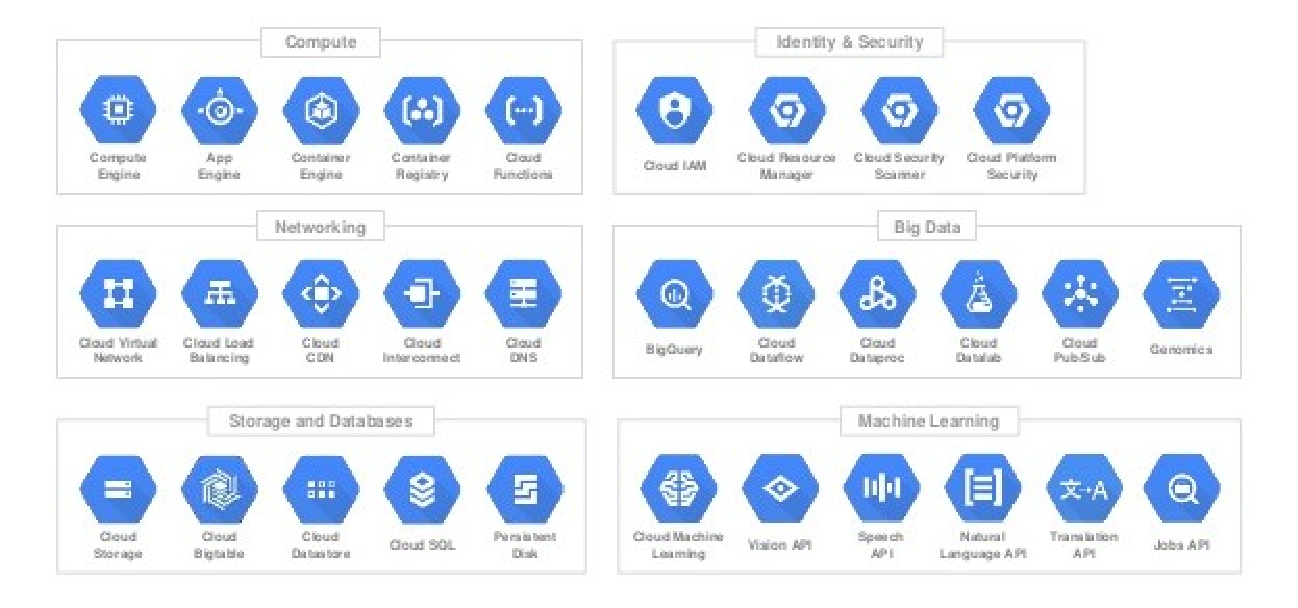
\includegraphics[scale=0.75]{imagens/google_cloud_services.eps}
  \caption{Serviços do Google Cloud\cite{googlecloudservices}}
\end{figure}

O Google Cloud possui quatro serviços essenciais de nuvem para aplicações, sendo eles: \textbf{App Engine}, \textbf{Compute Engine}, \textbf{Kubernetes Engine} e \textbf{Cloud Functions}. Além disso, possui toda a infraestrutura de gerenciamento de rede, banco de dados, \textit{big data}, \textit{machine learning}, entre outros.

\section{Funcionamento básico}

No contexto do documento, serão destacados os quatro serviços já citados anteriormente:

\begin{figure}[h!]
  \centering
  \includegraphics[scale=0.30]{imagens/google_cloud_dashboard.eps}
  \caption{Exemplo do \textit{Dashboard} do Google Cloud com seus recursos}
\end{figure}

\subsection{Cloud Functions}

As \textbf{Cloud Functions} têm como principal funcionalidade atender pequenos trechos de código, gerando \textit{endpoints} prontos para o usuário final utilziar. O produto atende em especial pessoas que não necessitam de grandes aplicações para solucionarem seus problemas, onde um microserviço seria algo elevado demais para o contexto.

O funcionamento básico dele consiste em implementar soluções simples no ambiente de microserviços sobre monólitos, explicado da seguinte forma pelo Google\cite{googlecloudfunctions}:

\begin{citacaoLonga}
  A agilidade do desenvolvedor vem de sistemas de construção compostos por pequenas unidades de funcionalidade independentes que executam uma única coisa muito bem. O Cloud Functions permite criar e implantar serviços no nível de uma única função, e não no nível de aplicativos, contêineres ou VMs inteiros.
\end{citacaoLonga}

Contextualizando, é possível subir simples funções e deixar o gerenciamento da escalabilidade com o próprio Google Cloud, facilitando a vida do desenvolvedor. Uma solução similar é implementada pela suíte de soluções da Amazon Web Services: as funções \textit{lambda}.

\subsection{App Engine}

O \textbf{App Engine} é um serviço intermediário, permitindo que aplicações completas sejam hospedadas em seu serviço, porém com os recursos necessários apenas e sem grandes preocupações em gerenciamento da escalabilidade.

Seu funcionamento consiste em hospedar aplicações completas no estilo \textit{PaaS} (\textit{Platform as a Service}), deixando de lado a parte de gerenciamento de infraestrutura para o Google Cloud. O depoimento abaixo, de Stefan Hauk,
Desenvolvedor da empresa de games Rovio, ilustra bem o funcionamento do serviço\cite{googlecloudappengine}:

\begin{citacaoLonga}
  Nossos jogos da Web tendem a ficar famosos imediatamente, então não temos a opção de escalonamento ao longo do tempo. O Google App Engine simplifica esse processo, já que ele pode iniciar instantaneamente quantos servidores forem necessários.
\end{citacaoLonga}

A vantagem do serviço está no escalonamento automático simples, o que facilita o trabalho do desenvolvedor. Alem disso, há uma integração tranquila com as principais linguagens de programação usadas, atendendo os mais diversos problemas de maneira simples. A solução é bem parecida com a implementada por padrão pelo Heroku.

\subsection{Kubernetes Engine}

O \textbf{Kubernetes Engine} é uma solução mais robusta que permite o uso de \textit{containers}, dando maior poder ao desenvolvedor para escalar sua aplicação em máquinas virtuais. A solução adotada pelo Google usa seu próprio orquestrador de \textit{containers}, o Kubernetes, definido pelo Google (em inglês)\cite{kubernetes}:

\begin{citacaoLonga}
  Kubernetes is an open-source system for automating deployment, scaling, and management of containerized applications. It groups containers that make up an application into logical units for easy management and discovery.
\end{citacaoLonga}

Seu funcionamento consiste em gerenciar \textit{containers} de acordo com as necessidades dos usuários, onde as aplicações colocadas em produção se encontram dentro deles. Essa ferramenta permite maior controle do desenvolvedor para determinar quantos e quais \textit{containers} serão escalados, para atender a demanda necessária.\nocite{googlecloudcontainerengine}

\subsection{Compute Engine}

Por fim, o \textbf{Compute Engine} é a solução mais poderosa fornecida pelo Google, onde é disponibilizada uma máquina completa para o usuário subir suas aplicações. A solução é da categoria \textit{IaaS} (\textit{Infrastructure as a Service}), provisionando infraestruturas de acordo com a necessidade do desenvolvedor.

Seu funcionamento se assemelha ao EC2 da Amazon Web Services, onde a essência está em fornecer máquinas completas ao usuário final, com os mais diversos sistemas operacionais (tanto Linux quanto Windows). A escalabilidade é possível, expandindo recursos da máquina de acordo com as necessidades, mas todo o trabalho fica ao encargo do desenvolvedor.\nocite{googlecloudcomputeengine}

\section{Outros serviços}

Além dos serviços básicos de aplicações, merecem destaque outros serviços:

\begin{itemize}
  \item Armazenamento: Bigtable (NoSQL), Cloud SQL (MySQL e PostgreSQL).
  \item Rede: Rede VPC (Gerenciamento de IP), Balanceamento de Carga.
  \item \textit{Stackdriver}: Monitoração, Depuração e Registros das Aplicações.
  \item Big Data: BigQuery (Análise de dados massivos), Dataflow (\textit{Pipeline} para processamento de dados), IoT Core (Mensagens em tempo real).
\end{itemize}

\section{Conclusão}

O Google Cloud possui uma suíte bem completa de produtos, para os mais diversos públicos e problemas a serem solucionados, tanto soluções auto-escaláveis quanto máquinas completas para aplicações mais complexas, tudo com a infraestrutura do Google e a preços mais acessíveis do que concorrentes como o Heroku.
